\section{Wahrscheinlichkeits Theorie}
\subsection{Ereignisse und ihre Wahrscheinlichkeit}
	\subsubsection{Kombinatorik}
		\begin{minipage}{13.5cm}
		\begin{tabular}{| p{5.5cm} | c | c |}
			\hline
			Art der Auswahl bzw. Zusammenstellung von $k$ aus $n$ Elementen
			& \multicolumn{2}{c|}{Anzahl der M�glichkeiten}\\
 			& ohne Wiederholungen		& mit Wiederholungen\\
 			& $(k\leq n)$ 				& $(k\leq n)$ \\
 			\hline
 			Permutationen & $P_n=n!(n=k)$ &
 			$P_n^{(k)}=\frac{n!}{k!}$ \\ & &\\
 			Kombinationen & $C_n^{(k)}=\binom n k$ &
 			$C_n^{(k)}=\binom{n+k-1} k$\\
 			& &\\
 			Variationen & $V_n^{(k)}=k!\binom n k$ & $V_n^{(k)}=n^k$\\
 			\hline
		\end{tabular}
		\end{minipage}
		\begin{minipage}{5cm}
		$\binom n k$ mit TR: \texttt{nCr(n,k)} \hspace{9.3mm}En\\
		\hspace*{19mm} \texttt{Kombinat(n,k)} De
		\end{minipage}
		\begin{list}{$\bullet$}{\setlength{\itemsep}{0cm} \setlength{\parsep}{0cm} \setlength{\topsep}{0.1cm}} 
         	\item \textbf{Permutationen}: Gegeben seien $n$ verschiedene Objekte. Dann gibt es $n!$
         	verschiedene Reihenfolgen in denen man diese Objekte anordnen
         	kann. \\
         	z.B.: $x,y,z;\quad x,z,y;\quad z,y,x;\ldots$
         % \item Permutation nennt man eine Anordnung von $n$ Elementen in einer Bestimmten
		%		Reihenfolge
		 	\item \textbf{Kombination}: Gegeben seien $n$ verschiedene Objekte. Dann gibt es $\binom n k$
		 	M�glichkeiten, daraus $k$ Objekte auszuw�hlen, wenn es nicht auf die Reihenfolge
		 	ankommt. \\
		 	z.B.: Wie viele verschiedene M�glichkeiten hat man beim Lotto, 6 Zahlen aus 49
		 	auszuw�hlen?
		 % \item Kombination nennt man eine Auswahl von $k$ Elementen aus $n$ Elementen
		 % 		ohne Beachtung der Reihenfolge
		  \item \textbf{Variation} nennt man eine Auswahl von $k$ Elementen aus $n$
		  		verschiedenen Elementen unter Beachtung der Reihenfolge
        \end{list}
        
\hrule
\vspace{5mm}
	\begin{minipage}{6.8cm}
	\subsubsection{Wahrscheinlichkeit}
		\begin{tabular}{ll}
			Wertebereich:
			& ${0}\le{P(A)}\le{1}$\\ \\
			Sicheres Ereignis:
			& $P(\Omega)=1$\\ \\
			unm�gliches Ereignis:
			& $P(\emptyset)=0$
		\end{tabular}
	\end{minipage}
		\begin{minipage}{11.2cm}
		\subsubsubsection{Rechenregeln}
			\begin{tabular}{ll}
				komplement�r Ereignis:
				&$P(\bar{A})=P({\Omega}\setminus{A})=1-P(A)$\\ \\
				Differenz der Ereignisse A und B:
				&$P({A}\setminus{B})=P(A)-P({A}\cap{B})$\\ \\
				Vereinigung zweier Ereignisse:
				&$P({A}\cup{B})=P(A)+P(B)-P({A}\cap{B})$
			\end{tabular}
		\end{minipage}
\vspace{1mm}
\hrule
	
	\subsubsection{Laplace-Ereignisse}
    	In einem endlichen Wahrscheinlichkeitsraum $\Omega$ haben alle
    	Elementarereignisse die gleiche Wahrscheinlichkeit.
    	\begin{center}
    	$P(A)=\dfrac{\left| A\right|}{\left|\Omega\right|}$
    	\end{center}


\hrule

	\subsubsection{Unabh�ngige Ereignise}
		Unabh�ngige Ereignisse $A$ und $B$ liegen vor, wenn:\\
    	\hspace*{8mm} $P(A\mid B)=P(A)$ \hspace{4mm} und \hspace{4mm}
    	$P(B\mid A)=P(B)$\\
    	erf�llt ist. F�r sie gilt\\
    	\hspace*{8mm} $P(A\cap B)=P(A)P(B)$\\
    	Die Tatsache, dass A eingetreten ist, hat keinen Einfluss auf die 
		Wahrscheinlichkeit von B.\vspace{1mm}

\hrule

	\subsubsection{Bedingte Wahrscheinlichkeit}
		Die Wahrscheinlichkeit f�r das Eintreten des Ereignisses $A$ unter der
		Bedingung, dass das Ereignis $B$ bereits eingetreten ist.
		\begin{center}
		$P(A\mid B)= \dfrac{P(A\cap B)}{P(B)}=\underbrace{\frac{P(A)\cdot
		P(B)}{P(B)}=P(A)}_{\text{nur wenn unabh�ngig}}$ 
		\end{center}

\hrule

	\subsubsection{Satz von Bayes}
		\begin{tabular}{ll}
		$P(B\mid A)=P(A\mid B) \cdot\dfrac{P(B)}{P(A)}$\vspace{1mm}
		\end{tabular}

\hrule
	\subsubsection{Totale Wahrscheinlichkeit }
		\begin{tabular}{ll}
        $P(A)=\sum\limits_{i=1}^N P(A\mid G_i)\cdot P(G_i)$
        \end{tabular}

\subsection{Erwartungswert und Varianz}

	\subsubsection{Erwartungswert }
		Sei $X$ eine Funktion auf $\Omega$, und lasse sich $\Omega$ in endlich viele
		Ereignisse, auf denen $X(\omega)$ konstant ist, $A_i$ zerlegen, dann ist der
		Erwartungswert von $X$\\
        \hspace*{5.7cm}$Erwartungswert = \sum Wert \cdot Wahrscheinlichkeit$\\
		\hspace*{7.5cm}$E(X)=\sum\limits_{i=0}^n \underbrace{X(A_i)}_{\text{Wert}}\cdot \underbrace{P(A_i)}_{\text{W'keit}}$

		\subsubsubsection{Rechenregeln}
			\begin{tabular}{ll}
    		$E(X+Y)=E(X)+E(Y)$\\
    		$E(\lambda X + \mu)=\lambda \cdot E(X) + \mu$ & $\lambda, \mu \in \mathbb{R}$\\
    		$E(XY) = E(X)\cdot E(Y)$ & wenn X,Y unabh�ngig sind\\
    		\end{tabular}

\vspace{1mm}
\hrule
\vspace{2mm}

	\begin{minipage}{9cm}
	\subsubsection{Varianz }
		\begin{tabular}{ll}
		$var(x)=\sigma ^2=E[(X-E(X))^2]=E(X^2)-E(X)^2$\\
		\end{tabular}

		\subsubsubsection{Kovarianz }
		\begin{tabular}{ll}
        $cov(X,Y)=E(XY)-E(X)E(Y)=\underbrace{0}_{\text{falls X,Y unabh�ngig}}$
        \end{tabular}
	\end{minipage}
		\begin{minipage}{9cm}
		\subsubsubsection{Rechenregeln}
			\begin{tabular}{ll}
        	$var(\lambda X)=\lambda^2 var(X) \qquad $ $\lambda, \mu \in
        	\mathbb{R}$\\ 
        	$var(X_1+X_2+\ldots+X_n) \neq var(n X)$ \\
        	$var(X+Y)= \begin{cases}
	                      var(X)+var(Y)
	                      &	\text{(X,Y unabh.)}\\                     
	                      var(X) + var(Y) + 2 \cdot cov(X,Y) 
	                      &	\text{(X,Y abh�ngig)}\\
                     \end{cases} $ \\
        	$var(X Y)= var(Y)var(X)+var(Y)E(X)^2+var(X)E(Y)^2$
        	\end{tabular}
		\end{minipage}
\vspace{1mm}

\hrule

		\subsubsection{Erwartungswert und Varianz des arithmetischen Mittels }
		Es sei eine folge von unabh�ngigen Zufallsvariablen $X_1, X_2, \ldots , X_n$ mit gleichem
		Erwartungswert $ \mu $ und gleicher Varianz $ \sigma^2 $ gegeben.  \\
		\begin{tabular}{p{6cm} p{6cm} p{6cm}}
	        Mittelwert: $M_n=\frac{X_1+\ldots+X_n}{n}$ 
	        & Erwartungswert: $E(X)=E(M_n)$
	        & Varianz: $var(M_n)=\frac{1}{n}var(X)$
        \end{tabular}
\vspace{1mm}

\hrule

\vspace{2mm}
	\begin{minipage}[]{9cm}
	\subsubsection{Regression }
		\begin{tabular}{ll}
        Allgemein: & X,Y Zufallsvariable\\
        Gesucht: & Regressionsgerade $y=ax+b$ mit min. Fehler\\
        Fehler: & $E(Y-(aX+b))=0$
        \end{tabular}
		\vspace{.1cm}

		\textbf{Regressionskoeffizient r}\\
        r ist ein Mass f�r die Qualit�t der Regression (standardisiert)\\
        $r^2=\dfrac{cov(X,Y)^2}{var(X)var(Y)}$ \\
        
		\textbf{Mittlerer quadratischer Fehler}\\
        $ \Delta^2 = var(Y)(1-r^2) =
        var(Y)\left(1-\dfrac{cov(X,Y)^2}{var(X)var(Y)}\right) $ \\
        
        \textbf{Berechnung mit Taschenrechner (TI-89, V-200)}
        \begin{list}{$\bullet$}{\setlength{\itemsep}{0cm}
        \setlength{\parsep}{0cm} \setlength{\topsep}{0cm}}  
	        \item Vorbereitung:\\
	        \texttt{$\{x_1, \ldots, x_n\} \blacktriangleright$\texttt{l1}$; \; 
	        \{y_1, \ldots,y_n\}\blacktriangleright$ \texttt{l2}$; \;$} \texttt{LinReg l1,l2}
	        \item Anzeige von Werten mit \\ \texttt{ShowStat}
	        \item Anzeige des Graphs mit \\
	        \texttt{reqeq(x)}$\blacktriangleright$\texttt{y1(x)}$; \;$
	        \texttt{NewPlot 1,1,l1,l2}
        \end{list}
	\end{minipage}
	\begin{minipage}{10cm}
    
	\textbf{Vorgehen:} \textcolor{grey}{mit Fehlerberechnung}
	\begin{enumerate}
		\item Tabelle mit bekannten Werten aufstellen:\\
		\begin{tabular}{|l||l|l||l|l||l|}
		\hline
		\textbf{$k$} & \textbf{$x$} & \textbf{$x^2$} & \textbf{$y$} &
		\textcolor{grey}{\textbf{$y^2$}} & \textbf{$xy$} \\ \hline \hline
		$1$ & $x_1$ & $x_1^2$ & $y_1$ & \textcolor{grey}{$y_1^2$} & $x_1y_1$ \\ \hline
		$\vdots$ & $\vdots$ & $\vdots$ & $\vdots$ & \textcolor{grey}{$\vdots$} &
		$\vdots$ \\\hline
		$n$ & $x_n$ & $y_n^2$ & $y_n$ & \textcolor{grey}{$y_n^2$} & $x_ny_n$ \\ \hline
		\hline
		$\sum$ & $\sum x_k$ & $\sum x_k^2$ & $\sum y_k$ & \textcolor{grey}{$\sum
		y_k^2$} & $\sum x_ky_k$ \\ \hline
		$E$ & $\frac{\sum x_k}{n}$ & $\frac{\sum x_k^2}{n}$ & $\frac{\sum y_k}{n}$ &
		\textcolor{grey}{$\frac{\sum y_k^2}{n}$} & $\frac{\sum x_ky_k}{n}$ \\ \hline
		\end{tabular} 

		\item Varianzen, Kovarianz berechnen:\\
		$var(X) = E(X^2) - E^2(X)$ \\
		\textcolor{grey}{$var(Y) = E(Y^2) - E^2(Y)$} \\
		$cov(X,Y) = E(XY) - E(X)E(Y)$
		\item Koeffizienten \textcolor{grey}{und Fehler} der Gerade berechnen:\\
		$a=\dfrac{cov(X,Y)}{var(X)}$
		\textcolor{grey}{$\qquad\Delta^2=var(Y)\left(1-\dfrac{cov(X,Y)^2}
		{var(X)var(Y)}\right) $}\\ $b=E(Y)-aE(X)$
		\item Gerade:\\
		$y=ax+b$
	\end{enumerate}
	\end{minipage}
\vspace{2mm}
\hrule
		
	\subsubsection{Satz von Tschebyscheff }
		\begin{tabular}{ll}
        $P(\left| X-E(X)
        \right|>\varepsilon)\leq\dfrac{var(X)}{\varepsilon^2}$ &
        Wahrscheinlichkeit, dass $X$ um mehr als $\varepsilon$ vom
        Erwartungswert $E(X)$ abweicht.\\
        \end{tabular}

\newpage

\subsection{Wahrscheinlichkeitsverteilung}
	\subsubsection{Verteilungsfunktion }
		\renewcommand{\arraystretch}{1.5}
		\begin{tabular}[]{|l|l|}
        	\hline
        	\textbf{diskret} & \textbf{kontinuierlich}\\
        	\hline
        	\hline
        	$P(X\leq x)=F(x)=\sum\limits_{k=-\infty}^x p_k$ &
        	$P(X\leq x)=F(x)=\int\limits_{-\infty}^x
        	\varphi(\tilde{x})d\tilde{x}$\\
  			$P(X>x)=1-P(X\leq x)$ & $P(X>x)=1-P(X\leq x)$\\        	
        	$P(a \le X \leq b)=F(b)-F(a)=\sum\limits_{k=a}^b p_k$ &
  			$P(a \le X \leq b)=F(b)-F(a)=\int \limits_a^b
  			\varphi(\tilde{x})d\tilde{x}$\\
        	\hline
        \end{tabular}
		\renewcommand{\arraystretch}{1}\\
	\subsubsubsection{Eigenschaften}
  				$$\boxed{\mathbb{D}(F) = \mathbb{R}} \qquad \boxed{\mathbb{W}(F)
  				\in[0,1]} \qquad \boxed{F(-\infty)=0} \qquad  \boxed{F(\infty)=1}
  				\qquad \boxed{F(x) \text{ ist monoton steigend}}$$

\hrule

\vspace{2mm}
	\begin{minipage}{13cm}
	\subsubsection{Wahrscheinlichkeitsdichte }
		\begin{tabular}{p{3.3cm}p{8.5cm}}
    	$\varphi(x)=F'(x)$ &Dichtefunktion oder Wahrscheinlichkeitsdichte\\
    	\multirow{2}{11cm}{Bei Sprungstellen von F(x): }\\
    	\multirow{2}{11cm}{$\varphi(x) = $ Dirac mit Gewichtung der Sprungh�he}
    	
    	\end{tabular}
	\end{minipage}
	\begin{minipage}{5cm}
		\subsubsubsection{Erwartungswert}
			\begin{tabular}{ll}
            $\textcolor{red}{E(}\textcolor{green}{X}\textcolor{red}{)}=
        	\textcolor{red}{\int} \textcolor{green}{x} \cdot 
        	\textcolor{red}{\varphi(x)dx}$\\
        	$\textcolor{red}{E(}\textcolor{green}{X^2}\textcolor{red}{)}=
        	\textcolor{red}{\int} \textcolor{green}{x^2} \cdot 
        	\textcolor{red}{\varphi(x)dx}$\\ 
        	$\textcolor{red}{E(}\textcolor{green}{X^N}\textcolor{red}{)}=
        	\textcolor{red}{\int} \textcolor{green}{x^N} \cdot 
        	\textcolor{red}{\varphi(x)dx}$\\ 
%         	$\textcolor{red}{E(}\textcolor{green}{\sin X}\textcolor{red}{)}=
%         	\textcolor{red}{\int} \textcolor{green}{\sin x} \cdot 
%         	\textcolor{red}{\varphi(x)dx}$
			
        	\end{tabular}
	\end{minipage}
\vspace{2mm}
\hrule
	\subsubsection{Rechenregeln f�r $\varphi$ und $F$}
		\begin{minipage}{11cm}
			\begin{tabular}{ll}
        	Gegeben: &X, Y Zufallsvariablen\\
        	&$\varphi_X$, $\varphi_Y$ bekannt\\
        	\end{tabular}
 
        	\begin{tabular}{p{6cm}p{6cm}}
        	Verteilungsfunktion: &Dichte:\\
        	$F_{X+a}(x)=F_X(x-a)$  &$\varphi_{X+a}(x)=\varphi_X(x-a)$\\
        	$F_{\lambda X}(x)=F_X(\frac{x}{\lambda})$ &$\varphi_{\lambda
        	X}(x)=\varphi_X(\frac{x}{\lambda})\frac{1}{\lambda}$\\
        	$F_{X+Y}(x)=F_X\ast\varphi_Y(y)=F_Y\ast\varphi_X(x)$ &
        	$\varphi_{X+Y}(x)=\varphi_X\ast\varphi_Y(x)$\\
        	$F_{\sqrt{X}}(x)=F_X(x^2)$ &
        	$\varphi_{\sqrt{X}}(x)=2x\varphi_X(x^2)$\\
        	$F_{X^2}(x)=F_X(\sqrt{x})$ &
        	$\varphi_{X^2}(x)=\frac{1}{2}x^{-\frac{1}{2}}\varphi_X(\sqrt{x})$
        	\end{tabular}
		\end{minipage}
		\begin{minipage}{7cm}
        	\subsubsubsection{Algorithmus Bsp.}
        	\begin{tabular}{ll}
        	1. Definition von $F$ anwenden: $F_{\lambda X}(x)=P(\underbrace
        	{\lambda X\leq x}_{*})$\\ 
        	2. Bedingung * umformen: $P(X \leq
        	\frac{x}{\lambda})=F_X(\frac{x}{\lambda})$\\ 
        	3. f�r Dichte: $\frac{d}{dx}$\\
        	\vspace{1mm}
        	$\varphi_{\lambda X}(x)=\frac{d}{dx}F_{\lambda
        	X}(x)=\frac{d}{dx}F_X(\frac{x}{\lambda})=
        	\varphi_X(\frac{x}{\lambda})\frac{1}{\lambda}$
        	\end{tabular}
			\vspace{7mm}
        \end{minipage}\\
		\subsubsubsection{Maximalwert eines Intervalls }
		$X_1,\ldots X_i$ sind auf dem Intervall $[0,l]$ mit $F_X(x)$ verteilt\\
		M=$\max \{ X_1,\ldots,X_i\} $\\
		$F_M(x)=F_X(x)^n$\\
\hrule
	\subsubsection{Normalverteilung}
		\begin{minipage}{10cm}
		Viele kleine, unabh�ngige Zufallsvariable sammeln sich zu einer
		normalverteilten Zufallsvariable.\\
		 $\varphi(x)=\frac{1}{\sqrt{2
		\pi}\sigma}\cdot e^{-\frac{(x-\mu)^2}{2\sigma^2}} = N(\mu ; \sigma^2) $\\ 
		$F(x)=\frac{1}{\sqrt{2
		\pi}\sigma}\cdot \int\limits^{x}_{-\infty}{e^{-\frac{(\tilde{x} -\mu)^2}{2\sigma^2}}} $ \\
		% = N(\mu ; \sigma^2),\tilde{x}} $
		\textbf{Standardisierung}\\
		Erwartungswert: $E(X)=\mu$ \hspace{4mm}(=0 bei Standardnormalver.)\\ 
		Varianz \hspace{11.5mm}: $var(X)=\sigma^2$ (=1 bei Standardnormalver.)\\ \\
		$x=\dfrac{X-\mu}{\sigma}$ \hspace{5mm} $x$ aus Tabelle
		\end{minipage}
		\begin{minipage}{8cm}
		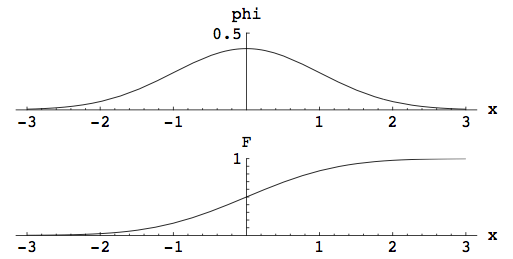
\includegraphics[width=8cm]{bilder/normalverteilung.png}
		Dichtefunktion (oben) und Verteilungsfunktion (unten) der Normalverteilung. 
   		\end{minipage} \\ \\
	$ 68\% $ der Werte liegen im Intervall $[ \mu - \sigma, \mu + \sigma]$, 
	$95\% $ in $[ \mu - 2\sigma, \mu + 2\sigma]$, 	
	$99.7\% $ in $[ \mu - 3\sigma, \mu + 3\sigma]$

	\subsubsection{Zentraler Grenzwertsatz }
      	$X_1, X_2, \ldots , X_n$ sind lauter identisch verteilte (nicht notwendig normalverteilt!)
      	unabh�ngige Zufallsvariablen mit demselben Erwartungswert $\mu$ und derselben Varianz $\sigma^2$.
      	\\ 
      	Dann hat die Summe ($S_n = \sum_{i=1}^n X_i$) den Erwartungswert $n \mu$ und die Varianz
      	$n \sigma^2$. \\
      	Die damit verbundene standardisierte ($E(X) = 0, var(X) = 1$) Variable $Z_n$ ist somit wie
      	folgt definiert: \\ $ Z_n = \dfrac{S_n - n \mu}{\sqrt{n} \sigma} = \dfrac{\overline{X} - \mu}{\sigma
      	/ \sqrt{n}}$
      	\\
      	F�r $\boldsymbol{n \to \infty}$ strebt die Verteilung von $Z_n$ gegen die
      	Standardnormalverteilung. \\
      	
      	
 \skriptsubsection{Maximum  a Posteriori}{28}
   Find the maximum a posteriori for a given a priori and density function for every value in $\mathcal{A}_i$:
   $$\max_i p_{Y | \mathcal{A}_i}(y) P(\mathcal{A}_i)$$
        
  \skriptsubsection{Maximum-Likelihood Estimation}{29}
  Maximum-Likelihood estimation tries to find an optimum solution if a parameter vector
  $\bm{\theta}$ is unknown.
  The likelihood of $\bm{\theta}$ with respect to the set of samples is defined as 
  $p(\mathcal{D} | \bm{\theta}) = \prod_{k=1}^{n} p(\mathbf{x}_k | \bm{\theta})$ 
  (samples are i.i.d. - independent \& identically distributed).
  
  \begin{minipage}{12cm}
	  Recipe with log-likelihood:
	  \begin{aufzaehlung}
	    \item Log-likelihood: $l(\bm{\theta}) = \ln (p(\mathcal{D} | \bm{\theta}))=\sum\limits_{k=1}^n \ln(p(\mathbf{x}_k | \bm{\theta}))$ \quad $\left( \frac{d}{dx} \ln(x) = \frac1x \right)$
	    \item Derivative: $\nabla_{\bm{\theta}} l = 
	      \sum\limits_{k=1}^n \nabla_{\bm{\theta}}\ln(p(\mathbf{x}_k | \bm{\theta}))$
	    \item Setting derivative to zero: $\nabla_{\bm{\theta}} l = 0$ and find solution 
	      $\bm{\hat{\theta}}=arg~ \underset{\bm{\theta}}{max}~ l(\bm{\theta})$
	  \end{aufzaehlung}
  \end{minipage}
  \begin{minipage}{8cm}
  	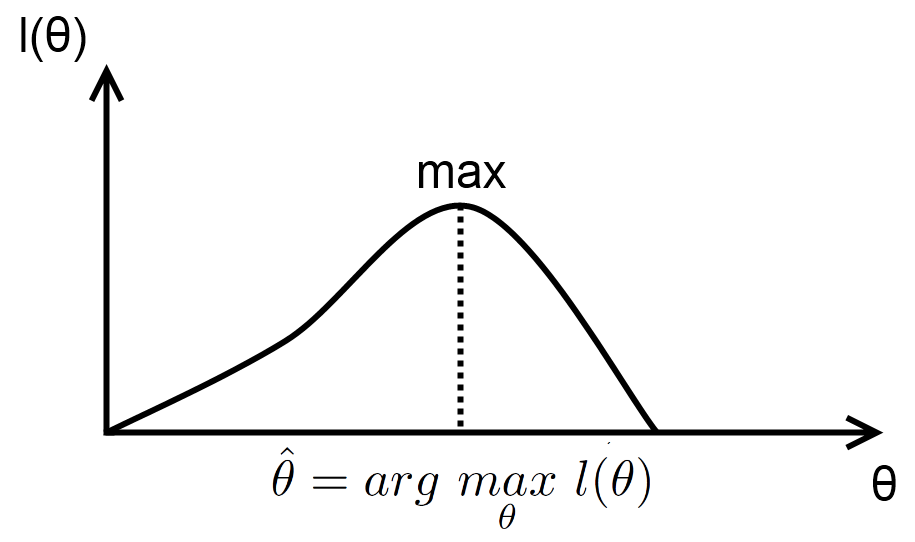
\includegraphics[width=7cm]{./bilder/MaxLikely.png}
  \end{minipage}
  